%
% wolframalpha.tex -- Integralbeispiel
%
% (c) 2021 Prof Dr Andreas Müller, OST Ostschweizer Fachhochschule
%
\bgroup
\begin{frame}[t]
\setlength{\abovedisplayskip}{5pt}
\setlength{\belowdisplayskip}{5pt}
\frametitle{$\displaystyle\int 1/(x^3 + 2x^2+x+1)\,dx$}
\begin{center}
\begin{tikzpicture}[>=latex,thick]
\uncover<1>{
\node at (0,0) {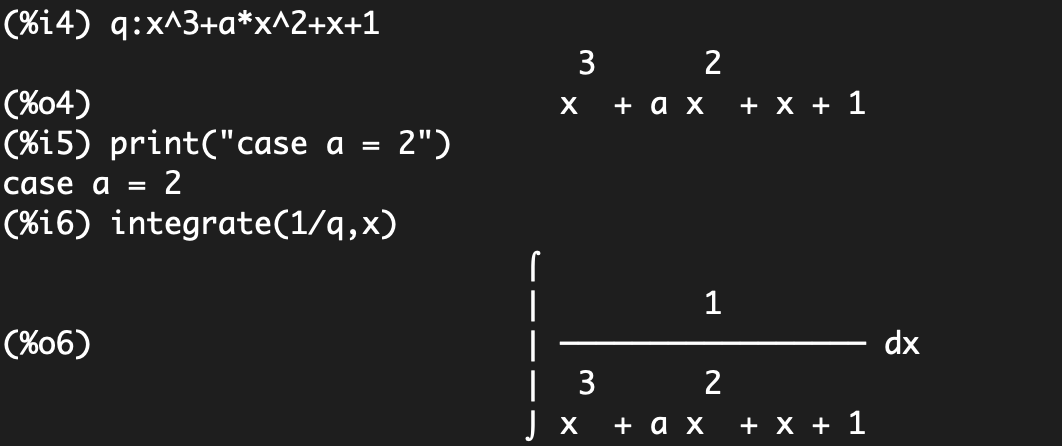
\includegraphics[width=13cm]{../slides/6/maxima.png}};
}
\uncover<2>{
\node at (0,0) {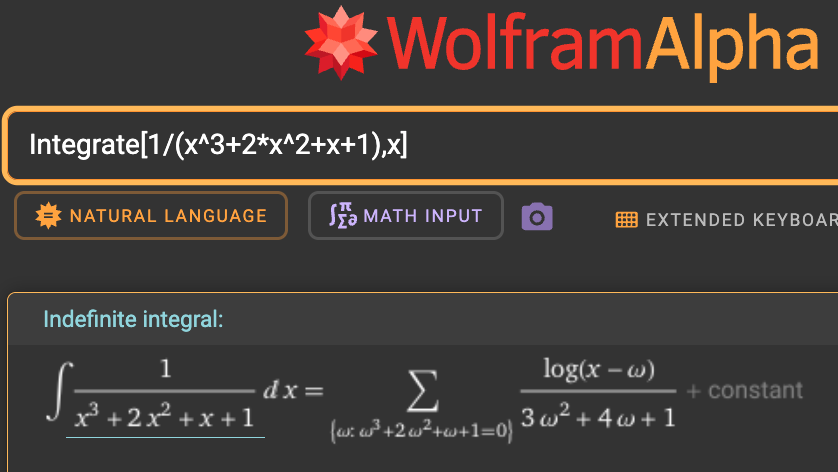
\includegraphics[width=13cm]{../slides/6/wolframalpha.png}};
}
\end{tikzpicture}
\end{center}
\end{frame}
\egroup
